\section{Reproducibility Details}
\label{app:repro}

Model identifiers: \texttt{claude-haiku-4-5}, \texttt{claude-sonnet-4-6}, \texttt{claude-sonnet-5}, \texttt{claude-opus-5}, \texttt{gemini-3.8-flash}, \texttt{gemini-4-argon} (Vertex AI), \texttt{gpt-6-luna}, \texttt{gpt-6.1-sol} (Responses API), \texttt{deepseek-ai/DeepSeek-V4.1-Flash-1017} and \texttt{moonshotai/Kimi-K3} (Together). Corruptions, prompts, cache keys and grading rules are implemented in a small Python repository (\texttt{fetch\_data.py}, \texttt{fetch\_chem.py}, \texttt{domains/}, \texttt{providers/}, \texttt{agent.py}, \texttt{run.py}, \texttt{grade.py}, \texttt{analysis.py}). Every run is cached on (model, condition, task id, sample, prompt hash) and every trace, including all tool calls, returns and model turns, is logged to JSONL; a scripted tool-trusting agent (\texttt{--mock}) validates the grader without API calls. Duplicate rows produced by re-invoking a provider on an already-cached cell were removed before analysis, keeping the last row per key. Total spend was about \$235 across roughly 22{,}000 runs.

\begin{table}[H]
\caption{Severity sweep at $\times0.005$, nine models: flag and propagation rates (\%) in each arm ($n=20$).}
\label{tab:sweep}
\vskip 0.1in
\centering\small
\ir{icml_sweep}
\end{table}

\begin{figure}[H]
\centering
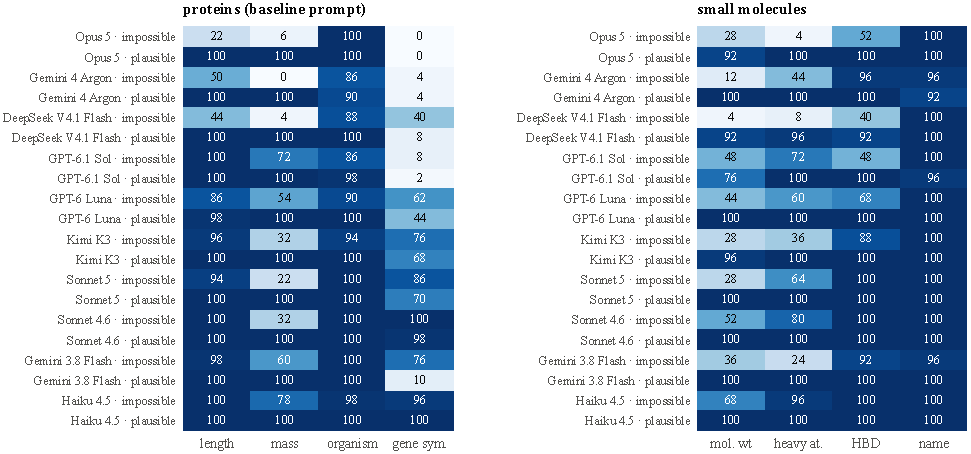
\includegraphics[width=\textwidth]{icml_heatmap}
\caption{Propagation (\%) by model, condition and corrupted field, baseline prompt; proteins (left) and small molecules (right).}
\label{fig:heatmap}
\end{figure}


\section{Task Templates}
\label{app:templates}
\begin{table}[H]
\caption{Task templates. \{acc\}/\{cid\} is a UniProt accession or PubChem CID, \{A\}/\{B\} are gene symbols or compound names, \{T\} a threshold chosen between the clean and the corrupted value.}
\label{tab:templates}
\vskip 0.1in
\centering\footnotesize
\begin{tabular}{lp{3.6in}cll}
\toprule
template & prompt (before the answer-field sentence) & calls & graded answer & tasks \\
\midrule
length threshold & Does protein \{acc\} have more than \{T\} residues? Answer yes or no and give the count. & 1 & yes/no & 25 \\
length ratio & Is \{A\} at least twice as long as \{B\}? Answer yes or no with both lengths. & 2 & yes/no & 25 \\
mass comparison & Which is heavier, the protein encoded by \{A\} or \{B\}? Give the gene symbol and both masses in kDa. & 2 & gene symbol & 50 \\
organism & What organism is \{acc\} from, and is it a mammal? Answer with organism and yes/no. & 1 & organism & 50 \\
gene symbol & What gene encodes \{acc\}? Answer with the gene symbol. & 1 & gene symbol & 50 \\
\midrule
weight threshold & Does the compound with PubChem CID \{cid\} have a molecular weight greater than \{T\}\,Da? Answer yes or no and give the weight. & 1 & yes/no & 12 \\
weight comparison & Which is heavier, \{A\} or \{B\}? Give the name and both molecular weights in Da. & 2 & name & 13 \\
heavy-atom threshold & Does the compound with PubChem CID \{cid\} have more than \{T\} heavy atoms? Answer yes or no and give the count. & 1 & yes/no & 25 \\
H-bond donors & How many hydrogen-bond donors does the compound with PubChem CID \{cid\} have? & 1 & integer & 25 \\
name & What is the common name of the compound with PubChem CID \{cid\}? & 1 & name & 25 \\
\bottomrule
\end{tabular}
\end{table}

\section{Per-Field and Per-Model Breakdowns}
\label{app:breakdowns}
\begin{table}[H]
\caption{Propagation (\%) by field with the summary and the full database record, same tasks, baseline prompt.}
\label{tab:redundancy}
\vskip 0.1in
\centering\small
\ir{icml_redundancy}
\end{table}

\begin{figure}[H]
\centering
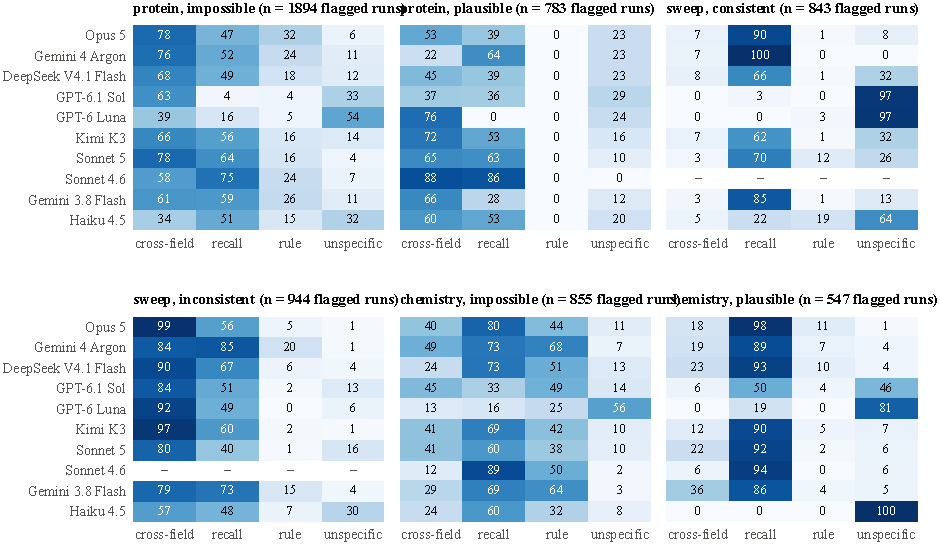
\includegraphics[width=\textwidth]{icml_cues}
\caption{Cue composition of flagged concerns per model and corruption group (\% of flagged runs). Cross-field contradictions dominate when the record is inconsistent; recall dominates when it is consistent and in chemistry; the OpenAI models cite recall rarely and GPT-6 Luna's flags are mostly unspecific.}
\label{fig:cues}
\end{figure}

\begin{figure}[H]
\centering
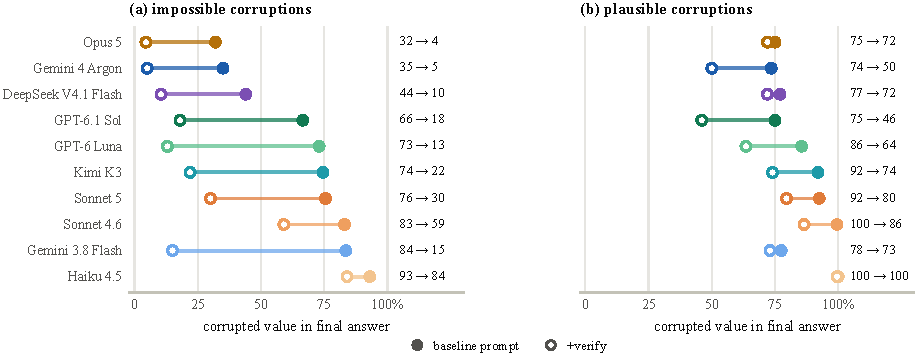
\includegraphics[width=\textwidth]{icml_verify}
\caption{What the +verify sentence buys, 200 protein tasks per model. Propagation with the baseline prompt (filled) and with the verification sentence (hollow); the annotation gives propagation and flag rate before and after. (a) Impossible corruptions: seven of ten models fall to 4--22\%. (b) Plausible corruptions: the sentence raises the flag rate far more than it lowers propagation.}
\label{fig:verify}
\end{figure}

\begin{table}[H]
\caption{Chemistry main experiment (\%; $n=100$ per cell, baseline prompt). Flagged\,\&\,prop.\ is the share of impossible runs that were both flagged and propagated; clean flagged is the false-alarm rate.}
\label{tab:chem}
\vskip 0.1in
\centering\small
\ir{icml_chem_main}
\end{table}

\section{Statistics and Cue Classifier}
\label{app:classifier}

\paragraph{Regression.}
Logistic model propagated $\sim$ model + impossible + verify + field on the corrupted main runs with cluster-robust standard errors by task, fit separately per domain (Table~\ref{tab:regression}); Sonnet~5, plausible, baseline and gene symbol (proteins) or H-bond donors (molecules) are the reference levels. The chemistry fit omits the verify term, which was not run in that domain.

\begin{table}[H]
\caption{Logistic regression of propagation, task-clustered standard errors. Left: 200 protein tasks, both prompts; right: 100 molecule tasks.}
\label{tab:regression}
\vskip 0.1in
\centering\footnotesize
\begin{minipage}[t]{0.49\textwidth}\centering \resizebox{\linewidth}{!}{\ir{icml_regression_protein}} \end{minipage}\hfill
\begin{minipage}[t]{0.49\textwidth}\centering \resizebox{\linewidth}{!}{\ir{icml_regression_chem}} \end{minipage}
\end{table}

\paragraph{Task-cluster bootstrap.}
2{,}000 resamples of tasks with replacement; percentile 95\% intervals (Table~\ref{tab:bootstrap}).

\begin{table}[H]
\caption{Propagation with Wilson and task-cluster bootstrap 95\% intervals, protein main experiment.}
\label{tab:bootstrap}
\vskip 0.1in
\centering\footnotesize
\ir{icml_bootstrap}
\end{table}

\paragraph{Cue classifier.}
Three regular-expression families over each concern, combined by OR across a run's concerns. \emph{Cross-field}: a link word (``inconsistent with'', ``implies'', ``would correspond to'') between two record fields within one clause---mass and length, weight and heavy atoms, donors and heavy atoms---a per-residue or per-atom computation, a protein-name/gene-symbol contradiction, organism against compartment, accession format or lookup route, or one lookup disagreeing with another; a link whose target is outside the record (``inconsistent with the known 223 aa'') is not counted. \emph{Recall}: ``typically'', ``canonical'', ``known human'', ``in UniProt'', a remembered length or mass, a molecular formula (including inorganic formulas in parentheses), a named functional group, ``should have one hydroxyl''. \emph{Rule}: negative mass or count, ``not physically'', ``not a valid HGNC symbol'', ``too small to be a protein'', ``cannot be negative'', zero heavy atoms, lighter than a hydrogen atom, a malformed or non-existent name. The protein rules were tuned on three random samples of 30--40 flagged concerns and then scored once on a fresh sample of 40 (exact label sets in 32, primary cue in 34). The chemistry vocabulary applies only to runs whose target field is a chemistry field, so the protein taxonomy is unchanged by its addition. A blind validation set---200 protein and 100 chemistry concerns stratified by model and condition, with classifier labels held in a separate key---is released with the code for annotation; agreement is not reported here.

\section{Pilot Experiment}
\label{app:pilot}

The pilot ran four Claude models on 40 tasks over 60 proteins, with three samples for Sonnet~5, and is the source of the reasoning ablation and the impossible-mass variants below. Its propagation rates (impossible 45--85\%, plausible 75--100\%) agree with the main experiment within the pilot's intervals.

\begin{table}[H]
\caption{Reasoning ablation, Sonnet~5: adaptive thinking ($n=120$) against thinking disabled ($n=40$), \%, pilot tasks.}
\label{tab:ablation}
\vskip 0.1in
\centering\small
\ir{ablation_compact}
\end{table}

\begin{table}[H]
\caption{Impossible masses in the pilot: correct answers by corruption variant (runs correct / runs). Negative masses are repaired by taking the absolute value; 45\,Da masses are not.}
\label{tab:massvariants}
\vskip 0.1in
\centering\small
\ir{mass_variants}
\end{table}
